\chapter{Parallelisierung}
\label{chp:para}

\begin{SCfigure}
  \centering
  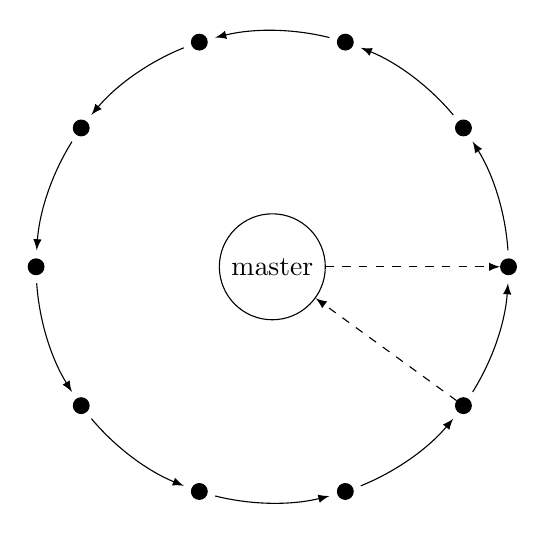
\begin{tikzpicture}
    [place/.style={circle,
      inner sep=0pt,minimum size=2mm}]
    %% from http://www.texample.net/tikz/examples/cycle/
    % Author : Jerome Tremblay
    \def \n {10}
    \def \radius {3cm}
    \def \margin {4} % margin in angles, depends on the radius

    \foreach \s in {1,...,\n}
    {
      \node[draw, circle, fill=black, place] (\s) at ({360/\n * (\s - 1)}:\radius) {};
      \draw[->, >=latex] ({360/\n * (\s - 1)+\margin}:\radius)
      arc ({360/\n * (\s - 1)+\margin}:{360/\n * (\s)-\margin}:\radius);
    }

    \node[draw, circle] (master) at (0:0) {master};
    \draw[->, >=latex, dashed] (master) -- (1);
    \draw[->, >=latex, dashed] (\n) -- (master);
  \end{tikzpicture}
  \caption[Mehrere Subpopulationen]{\label{fig:mult-subpop}Es werden mehrere Subpopulationen
    erzeugt, die dem jeweils nächsten Prozess dann Teile aus der
    eigenen Population zusenden.}
\end{SCfigure}

\begin{SCfigure}
  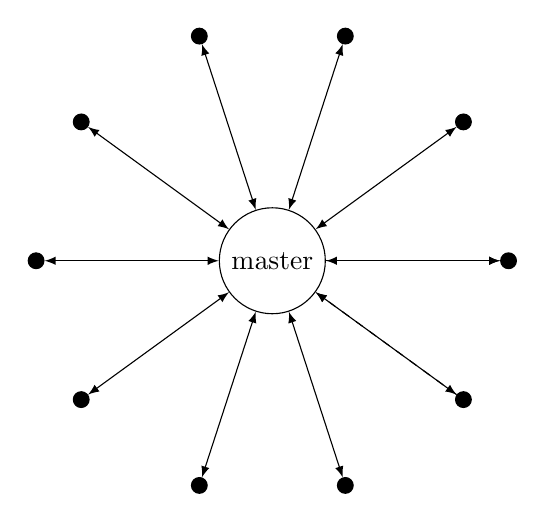
\begin{tikzpicture}
    [place/.style={circle,
      inner sep=0pt,minimum size=2mm}]
    \def \n {10}
    \def \radius {3cm}
    \def \margin {4} % margin in angles, depends on the radius

    \node[draw, circle] (master) at (0:0) {master};

    \foreach \s in {1,...,\n}
    {
      \node[draw, circle, fill=black, place] (\s) at ({360/\n * (\s - 1)}:\radius) {};
      \draw[<->, >=latex] (master) -- (\s);
    }

    \draw[->, >=latex, dashed] (master) -- (1);
    \draw[->, >=latex, dashed] (\n) -- (master);
  \end{tikzpicture}
  \caption[Verteilte Erzeugung von Offsprings]
  {\label{fig:topology-central} Die Kindprozesse erzeugen einzelne
    Rundreisen und schicken diese an den „master“ zurück.  Dieser muss
    die Rundreisen dann in die eigene Population einsortieren.}
\end{SCfigure}
